% !TeX spellcheck = es_ES
\documentclass[a4paper,12pt]{article}
\usepackage[utf8]{inputenc}
\usepackage{graphicx}
\usepackage{float}

%opening
\title{Maquina de Turing que duplica la cantidad de unos}
\author{Barrera Pérez Carlos Tonatihu \\ Profesor: Genaro Juárez Martínez \\ Computing Selected Topics \\ Grupo: 3CM8 }

\begin{document}

\maketitle
\newpage
\tableofcontents
\newpage
\section{Introducción}
\begin{center}
\begin{tabular}{|c|c|c|c|c|}
\hline
& \multicolumn{4}{|c|}{Simbolo} \\ \hline
Estado & 1 & X & Y & B\\ \hline
0 & (1, X, R) & - & (3, 1, R) & -\\ \hline
1 & (1, 1, R) & - & (1, Y, R) & (1, Y, L)\\ \hline
2 & (2, 1, L) & (0, 1, R) & (2, Y, L) & -\\ \hline
3 & - & - & (3, 1, R) & - \\ \hline
\end{tabular}
\end{center}
tabla
\begin{figure}[H]
\begin{center}
 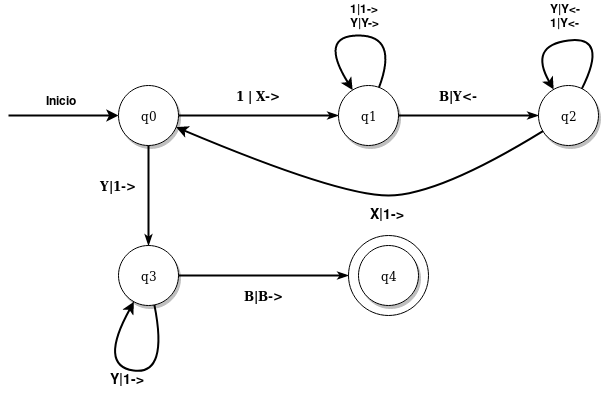
\includegraphics[width=12cm, height=7cm]{Turing-unos.png}
 \caption{Representación grafica de las transiciones de la maquina de Turing}
 \label{fig:diagrama4}
\end{center}
\end{figure}
\section{Desarrollo}
\section{Pruebas}

\end{document}
